\setcounter{figure}{0}

\section{12th November 2023 : I AM the vine, you are the branches}
\subsection*{Text: John 15:1-17}
  \begin{quote}
    [1] “I am the true vine, and my Father is the vinedresser. [2] Every
    branch in me that does not bear fruit he takes away, and every branch
    that does bear fruit he prunes, that it may bear more fruit. [3] Already
    you are clean because of the word that I have spoken to you. [4] Abide in
    me, and I in you. As the branch cannot bear fruit by itself, unless it
    abides in the vine, neither can you, unless you abide in me. [5] I am the
    vine; you are the branches. Whoever abides in me and I in him, he it is
    that bears much fruit, for apart from me you can do nothing. [6] If
    anyone does not abide in me he is thrown away like a branch and withers;
    and the branches are gathered, thrown into the fire, and burned. [7] If
    you abide in me, and my words abide in you, ask whatever you wish, and it
    will be done for you. [8] By this my Father is glorified, that you bear
    much fruit and so prove to be my disciples. [9] As the Father has loved
    me, so have I loved you. Abide in my love. [10] If you keep my
    commandments, you will abide in my love, just as I have kept my Father’s
    commandments and abide in his love. [11] These things I have spoken to
    you, that my joy may be in you, and that your joy may be full.

    [12] “This is my commandment, that you love one another as I have loved
    you. [13] Greater love has no one than this, that someone lay down his
    life for his friends. [14] You are my friends if you do what I command
    you. [15] No longer do I call you servants, for the servant does not know
    what his master is doing; but I have called you friends, for all that I
    have heard from my Father I have made known to you. [16] You did not
    choose me, but I chose you and appointed you that you should go and bear
    fruit and that your fruit should abide, so that whatever you ask the
    Father in my name, he may give it to you. [17] These things I command
    you, so that you will love one another.
  \end{quote}
\subsection*{Notes}
\begin{itemize}
  \item{This sunday is the last of the seven ``I AM'' statements. The first
  five ``I AM'' statements are to the crowd, they are: bread of life, light
  of the world, door, good shepherd, resurrection and the life. The last two
  are privately addressed to the disciples during Jesus' final word and
  prayer to his disciples before his arrest. The last two are: ``I AM the
  way, the truth and the life'', preached at gospel sunday two sundays ago.
  Today is ``I AM the true vine''.}
  \item{First part of the sermon: v1-v8.}
  \item{This is the only ``I AM'' statement where God the Father is
  mentioned. In the OT, the Father is portrayed as the vinedresser, and
  Israel is His vineyard. E.g Isaiah 5. And as we know in that passage, the
  vineyard was eventually taken away because it didn't bear good fruit. So
  here, Jesus said that He has replaced the vineyard (Israel) by being the
  \textbf{true vine}, and then believers who are in Jesus (who is the true
  vine) will be the true vineyard that produces fruit that God wants.}
  \item{Can our understanding of the OT metaphor of the vineyard and God the
  vinedresser be applied wholesale to our text in John? Note that in the OT,
  the covenant between Israel and God was based on works, but in the NT, we
  know we are justified by faith.}
  \item{In v3, Jesus says that the disciples were already clean because of
  the word that Jesus spoke. When Jesus spoke here, Judas had already gone
  out. What does He mean here? From the rest of the scripture, we see that
  this probably means that the disciples were justified by faith. But Judas
  also listened to the words that Jesus spoke. But Judas wasn't clean because
  of their unbelief.}
  \item{The 11 disciples will bear the good fruit in time, as they abide in
  Jesus. While Jesus will be taken up to heaven, He will be with His
  disciples through the Holy Spirit. On the other hand, Judas will be pruned
  away, because as will be seen, he will bear the bad fruit of betrayal. So from the 11 disciples and Judas, we can see the first example of
  what Jesus means here.}
  \item{Pastor Ronnie's view: from this text, we see that the pruning happens
  before any fruit is produced. This is a little different from the vineyard
  analogy in the OT, where the pruning happens after God has judged that
  Israel has bore no fruit. }
  \item{Note that the ``abide'' in v5 is in the present participle tense, and
  the ``abide'' in v6 is in the aorist tense. In v6, of which Judas is the
  prime example, Judas does not abide at all, it is not that he stops
  abiding, this is the sense of the aorist. Thus, our text here is not about
  how we need to continue abiding in Jesus if not we will be thrown away
  (since the pruning happens before fruit is borne). It is more about how
  those who abides in Jesus will bear much fruit. And one abides in Jesus by
  believing in the word that Jesus has spoken (v3, v7). In v3, we see that we
  are made clean by believing in the words that Jesus has spoken, and in v7,
  we see that when Jesus' words abide in us, God answers our prayers, which
  is a sign of God's relationship with us.}
  \item{Also, when we bear much fruit by abiding in Jesus, it is not to
  compare with each other or what. Jesus has previously said elsewhere that
  some would be given $10$ talents, some would be given $100$ talents; what
  is important is not the amount of fruit we bear, it is the faithfulness to
  God's spiritual graces in our life that is important. In the end, what is
  important is glorifying God. \KH{My own example: an illiterate person who
  believes in Jesus but is unable to do much because of his/her being
  illiterate as compared to a highly educated person like Tim Keller who
  writes many books to teach others. The illiterate person would still
  glorify God in his/her own way just by his/her simple faith!} }
  \item{There are people who appear to bear fruit, but actually their fruit
  is not fruit. These are people like Judas. We need to know God's word, so
  we can accurately discern what is true fruit, and what is not true fruit.
  This is important not so much for judging other people, but for examining
  ourselves. Is the fruit we are bearing true fruit? E.g, we might give to
  the poor, but it might be to brag for others. Or we might do good works,
  but it is to attempt to justify ourselves before God. If our fruit is not
  true fruit, then maybe we need to consider whether we have even started
  abiding in Jesus in the first place.}
  \item{We also see that the reason we are to bear fruit is to glorify God.
  If God is not glorified by the fruit you bear, then that is not
  faithfulness! This means that we should not have a secret faith, but we
  should speak openly and broadly about God's love for us which motivates us
  to bear the good fruit that we bear.}
  \item{Second part of the sermon: v9-v17.}
  \item{Two things that we learn here: we see that Jesus spoke these words so
  that Jesus' joy may be in the eleven disciples, and that their joy may be
  full. Based on the preceding text, we see that this joy has to do with
  love.}
  \item{Imagine if us Christians bearing fruit is solely for God's glory, as
  if we are servants serving a master. Such an attitude could be joyless. We
  see that Jesus laid down His life for the world because of His love for the
  Father, and the Father's love for Him (v9-10). This is the love that Jesus
  abides in, and which doesn't make sense to the world (it doesn't make sense
  to the world for Jesus to be crucified according to God's foreknowledge out
  of a mutual love between Jesus and the Father.) And this is the love that
  Jesus invites His disciples to partake in. }
  \item{And not only does Jesus lay down His life for the world because of
  His love for the Father, but He does so also because of His love for his
  disciples, whom he refers to as friends. Note: some commentaries argue
  whether it is greater for one to lay down one's life for his enemies, or
  for his friends. A simple answer is that such a self-sacrificial love would
  turn enemies into friends anyway. Even while we were ungodly, Jesus died
  for us (Romans 5), and this love of His so transforms us that our enmity
  towards Jesus transforms into us being disciples of Jesus, and thus Jesus'
  friends.}
  \item{Hence, our joy can be full, when we share in Jesus' love for His
  Father and His Father's love for Jesus, and when we understand Jesus' love
  for us. Abd we can share in this love by abiding in Jesus and bearing much
  fruit. The most important way to bear much fruit for God is to obey Jesus'
  commandments, of which the principal commandment given here is to love one
  another just as Jesus loves them. Note that this is not at odds with the
  great commandment, which is for us to love God and to love our neighbours
  as ourselves. Some might say that we must love not only Christians, but non-Christians too. That is true, but that does not contradict what Jesus says here. For the eleven disciples, their closest neighbours are each
  other. And for us, our closest neighbours are those at church. When we love
  each other in church, we are a powerful witness to the world. This powerful
  witness to the world is a form of loving our non-Christian neighbours. And
  when we love each other in church, we support each other in the struggles of loving our non-Christian neighbours. If we can't even love our Christian neighbours, then it is impossible for us to love our non-Christian neighbours! }
  % \item{\begin{figure}[H]
  %   \centering
  %   % 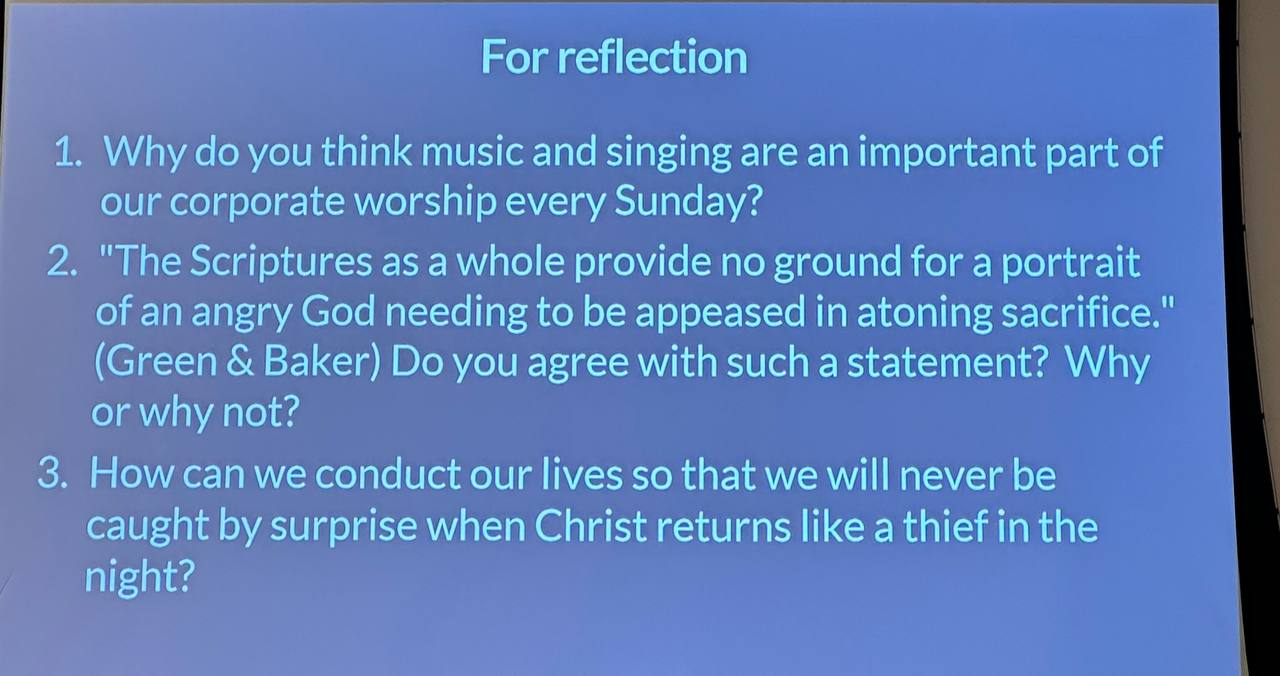
\includegraphics[width=0.8\textwidth, trim={0cm 0cm 0cm 0cm},clip]{Figures/marchSermon4Reflections.jpg}
  %   \includegraphics[width=0.8\textwidth, trim={0cm 0cm 0cm 0cm},clip]{example-image-a}
  %   \caption[]{Reflection questions for this sermon}
  %   \label{}
  % \end{figure}}
\end{itemize}